\documentclass{article}

% if you need to pass options to natbib, use, e.g.:
%     \PassOptionsToPackage{numbers, compress}{natbib}
% before loading neurips_2021

% ready for submission
\usepackage[nonatbib,preprint]{neurips_2021}

% to compile a preprint version, e.g., for submission to arXiv, add add the
% [preprint] option:
%     \usepackage[preprint]{neurips_2021}

% to compile a camera-ready version, add the [final] option, e.g.:
%     \usepackage[final]{neurips_2021}

% to avoid loading the natbib package, add option nonatbib:
%    \usepackage[nonatbib]{neurips_2021}

\usepackage[utf8]{inputenc} % allow utf-8 input
\usepackage[T1]{fontenc}    % use 8-bit T1 fonts
\usepackage[colorlinks=true]{hyperref}       % hyperlinks
\usepackage{url}            % simple URL typesetting
\usepackage{booktabs}       % professional-quality tables
\usepackage{amsfonts}       % blackboard math symbols
\usepackage{nicefrac}       % compact symbols for 1/2, etc.
\usepackage{microtype}      % microtypography
\usepackage{xcolor}         % colors
\usepackage{graphicx}

\title{Predicting Political Parties\\ from Text}

% The \author macro works with any number of authors. There are two commands
% used to separate the names and addresses of multiple authors: \And and \AND.
%
% Using \And between authors leaves it to LaTeX to determine where to break the
% lines. Using \AND forces a line break at that point. So, if LaTeX puts 3 of 4
% authors names on the first line, and the last on the second line, try using
% \AND instead of \And before the third author name.

\author{%
  Mattia Masiero\\
  Matrikelnummer 6100692\\
  \texttt{mattia.masiero@student.uni-tuebingen.de} \\
  \And
  Tim Weiland\\
  Matrikelnummer 6010188\\
  \texttt{tim.weiland@student.uni-tuebingen.de} \\
}

\begin{document}

\maketitle

\begin{abstract}
  The aim of this project was to predict political party affiliation from speeches held in the German Bundestag, sourced from the ParlSpeech data set. This project arose in the context of the lecture Data Literacy (WS 2021/22) at the University of Tübingen. The spirit of this project was to try out different methods and techniques for data analysis, to reflect on them in light of the lecture and to document results. The project comprised all stages of data analysis, starting from data retrieval, to preprocessing, analysis and visualization. Our final classification pipeline consists of preprocessing, feature extraction and logistic regression. In this setting, our model is three times as good at predicting political parties as chance. The resources associated with this project are accessible via a \href{https://github.com/timweiland/bundestag_party_prediction}{GitHub repository}.
\end{abstract}

\section{Data Set}
The ParlSpeech V2 data set \cite{DVN/L4OAKN_2020} comprises parliamentary speeches held in various representative democracies including Germany. The German record stems from the Dokumentations- und Informationssystem für Parlamentsmaterialien (DIP), which is the official and publicly accessible information system of the German Bundestag and Bundesrat. The release note of the data set explains, “Technically an individual speech (row) in our corpora refers to a continuous bit of text that was spoken on the plenary floor and that was clearly assigned to one and only one individual speaker as marked in the respective data source.” The data ranges from 1991-03-12 to 2018-12-14 and encompasses 379.545 speeches. The features of the data are: date, speech number (within the day at the parliament), speaker, party, chair (boolean; True if the speech was given by the chairperson of the Bundestag), terms (length of the speech in words), agenda, text.

\section{Preprocessing}
The raw data comes in R’s .rds format. As a first step we converted it to .csv, as this is easier to handle with Python. In line with the goal of our project, we removed all features except for the speeches and the corresponding parties. We then removed rows with “NaN” values, speeches which were given by the chairperson of the Bundestag, and speeches by MPs of “independent” party affiliation, since they do not represent one single party. Thus, the remaining parties were CDU/CSU, SPD, FDP, GRUENE, PDS/LINKE and AfD. The speeches themselves required some light preprocessing, as they still contained comments by other MPs, and faulty punctuation characters.

The extraction of features from the texts was a crucial step in our project. One natural way of extracting features from a text is the Bag-of-Words-method. Simply put, each word in the vocabulary of the entire data set becomes a predictor in the model. Some words, which are on a list of “stop words” are discarded. Stop words are words which are regarded as insignificant, e.g. articles. For a data point (speech), the value of each predictor (word) is the absolute frequency of its occurrences within the speech. We also decided to discard words that appear in more than 50\% of the speeches as they are effectively also stop words.

Since the Bag-of-Words-approach does not capture the structure of a text, we aimed at extracting another set of features, which capture some of its structural qualities, and use them as predictors alongside the Bag-of-Words predictors. The goal was both to improve prediction performance of the model and to gain insight over interpretable quantities. The 10 features we added are: Text length (in characters), average sentence length (in characters), number of profanities (based on a list aggregated from various sources), type-to-token-ratio (number of unique words vs. number of total words), average word length, fraction of stop words vs. non stop words, number of “!” and “?”, average tfidf-score (a measure of word importance obtained by combining a word's frequency within a document with its inverse frequency across all documents \cite{jonesStatisticalInterpretationTerm1972}), readability (calculated as Flesch-Reading-Ease for the German language), sentiment (calculated as the average sentiment of words in the speech; the sentiment scores stem from the SentiWS data set provided by the University of Leipzig \cite{remquahey2010}). Many of these features can be viewed as indicators of sophistication.

\section{Analysis}
\subsection{Models}
First, we split the data set into a training and a test set such that the test set takes up 10\% of the data set. To ensure that both data sets have a similar party distribution, we used stratified sampling. To build a classifier, we combined our hand-engineered features with the Bag-of-Words features into one sparse matrix, scaled all features such that they had unit variance, and then performed logistic regression with $\mathcal{L}_2$ regularization. We experimented with different approaches and hyperparameters and selected the best model via cross-validation on the training set.

\begin{table}[]
\center{
\begin{tabular}{|l|l|}
\hline
\multicolumn{1}{|c|}{\textbf{Method}} & \multicolumn{1}{c|}{\textbf{Accuracy}} \\ \hline
Only hand-engineered features         & 34.1\%                                 \\ \hline
Only Bag-of-Words features            & 53.8\%                                 \\ \hline
Hand-engineered + Bag-of-Words, naive & 54.3\%                                 \\ \hline
Hand-engineered + Bag-of-Words, fair  & 50.2\%                                 \\ \hline
\end{tabular}
}
\caption{Comparison of the test set accuracies of the different methods.}
\label{tab:method_comp}
\end{table}

We tried three different approaches based on which features are used for logistic regression: All features, only hand-engineered features and only Bag-of-Words features. For Bag-of-Words, we experimented with different vocabulary sizes (obtained by only keeping the top $k$ most frequent words), different optimization algorithms and numbers of iterations. Table \ref{tab:method_comp} shows the results for the initial three approaches as well as another approach which we will motivate in the following section. We see that Bag-of-Words is already extremely powerful on its own compared to the hand-engineered features. However, adding the hand-engineered features slightly increases the accuracy, hence they are not completely redundant. Nevertheless, we would have expected a more substantial performance increase due to their addition to the model.

We also tried using Principal Component Analysis and Latent Dirichlet Allocation to reduce the dimensionality of the Bag-of-Words features. We expected this to improve performance while yielding interpretable latent representations (that represent common topics), but we found that plain Bag-of-Words with regularized logistic regression always outperformed these methods.



\subsection{Intra-Class Performance and Fairness}
\begin{figure}
  \center{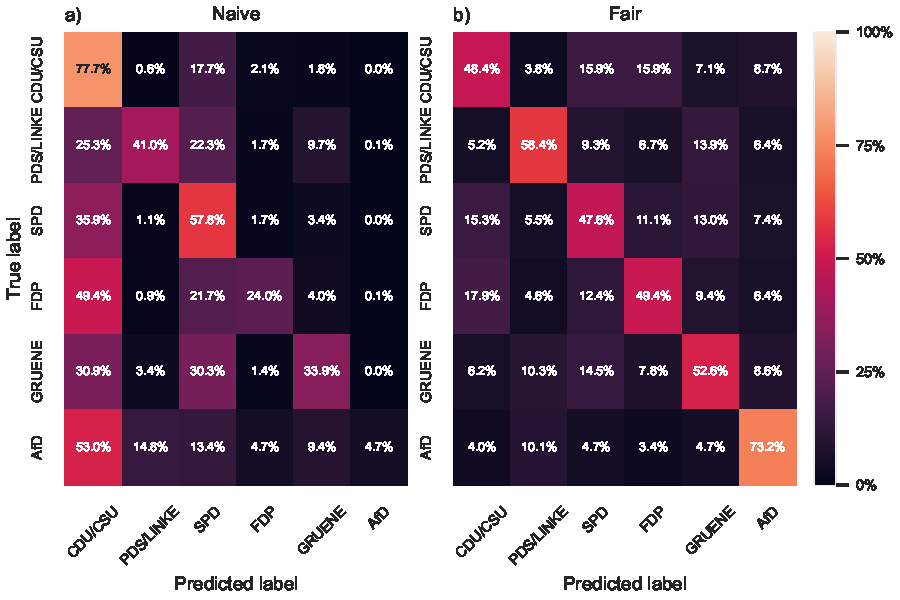
\includegraphics[width=1.0\textwidth]
  {figures/confusion_matrix_naive_vs_fair.pdf}}
  \caption{A comparison of the naive classifier and the fair classifier based on their confusion matrices. Entry $(i, j)$ of each confusion matrix contains the frequency with which the corresponding classifier classified a speech from party $i$ to belong to party $j$, normalized by the total number of speeches for party $i$.}
  \label{fig:conf_mat_comp}
\end{figure}


In this section we analyze the classifier's performance for each individual party. The confusion matrix in figure \ref{fig:conf_mat_comp}a shows the relative frequencies of all combinations of true label and predicted label. For instance, $35.9\%$ of all SPD speeches were incorrectly classified as CDU/CSU speeches. The diagonal thus contains the intra-class accuracies. We see that the classifier's performance is heavily biased towards the larger parties. This can be explained with the fact that the parties in the data set are not uniformly distributed: The data set is made up of speeches by 32.9\% CDU/CSU, 28.0\% SPD, 14.7\% GRUENE, 12.9\% FDP, 10.8\% PDS/LINKE and 0.7\% (!) AfD.

We would prefer a more balanced / ``fair'' classifier. To this end, we have decided to use weighted logistic regression. With this approach, in the loss function for logistic regression each sample is weighted by the inverse frequency of its corresponding party. We reused the hyperparameters we found for our original approach for this new approach and achieved a slightly lower accuracy of 50.2\%. Figure \ref{fig:conf_mat_comp}b shows the confusion matrix of the new classifier. We see that it is substantially more balanced and that it achieves acceptable intra-class accuracies for all classes.

\subsection{Similarities between Parties}
To evaluate the performance of our new classifier in an intuitive manner, we examine the largest off-diagonal entries of its confusion matrix in figure \ref{fig:conf_mat_comp}b. These correspond to parties that it mistakes for each other the most. The intuitive expectation is that these are parties that are similar to each other. This mostly holds true: Pairs that are often confused with another are CDU/CSU and FDP, CDU/CSU and SPD, GRUENE and LINKE. Curiously, we also see that AfD gets confused for LINKE in a non-negligible proportion, despite them being on opposite ends of the political spectrum. We argue that it is precisely the fact that they are on the extreme ends of the spectrum that makes them slightly similar: They are both in the opposition and frequently have views that are contrary to the majority, so we expect them to be more confrontational in their speeches.

\subsection{Out-of-Distribution Performance}
To test our classifier's out-of-distribution performance, we evaluated it on each party's 2021 manifesto. Each manifesto is a PDF document from which we extract the words (extracting sentences is difficult because of formatting, e.g. multiple columns per page). We then preprocessed the text as usual and replaced the missing features that depend on sentence structure with their respective global means in the ParlSpeech data set. Finally, we passed the processed data to the trained classifier. Our classifier achieved 100\% accuracy, i.e. all manifestos are classified correctly.

\subsection{Coefficient Visualization}
\begin{figure}
  \center{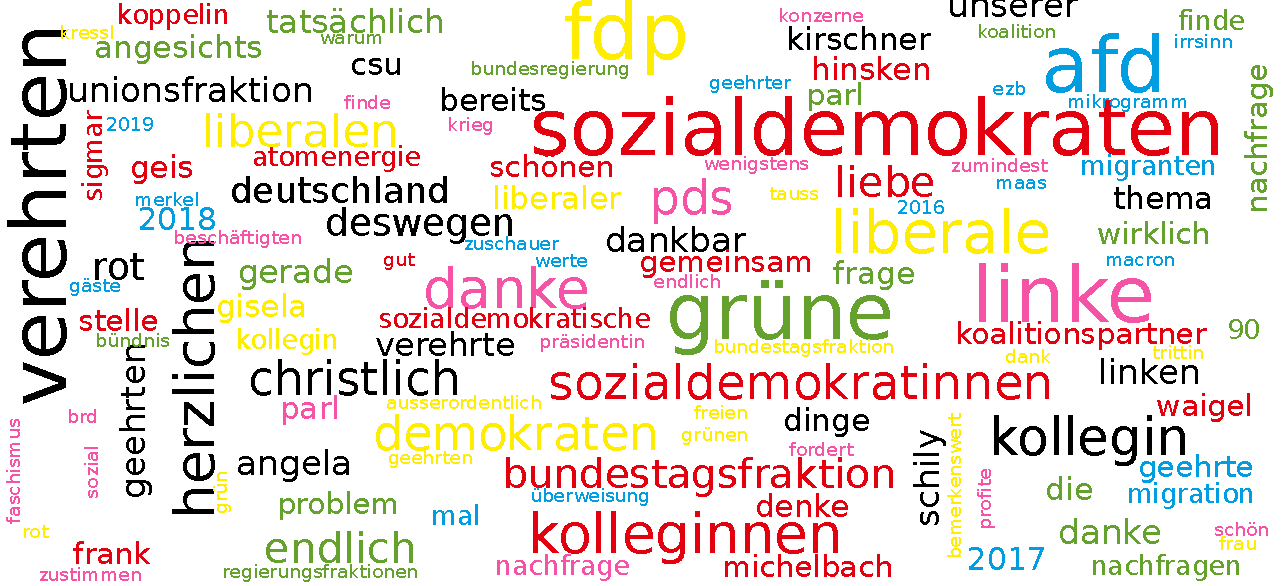
\includegraphics[width=1\textwidth]
  {figures/word_cloud.pdf}}
  \caption{The 20 largest coefficients for each party. The word colors correspond to the party colors, i.e. CDU/CSU: black, SPD: red, FDP: yellow, GRUENE: green, LINKE/PDS: magenta, AFD: blue.}
  \label{fig:wordcloud}
\end{figure}

Logistic regression with $n$ classes learns one set of weights for each class (i.e. party). To gain insight into the model, we decided to visualize for each party the features (i.e. words) with the largest coefficients. An intuitive and easily interpretable method is a “word cloud” plot, where the size of each word is proportional to the size of the coefficient, and the color of the word corresponds to the political party, see figure \ref{fig:wordcloud}. Note that the weights have been normalized for each party, such that the largest word for each party has the same size. As with any regression model, caution is due when interpreting the magnitude of the weights, since correlations between features distort the picture.

\section{Conclusion}
We argue that we have achieved satisfactory results that are substantially better than pure guessing. It can be difficult even for humans to predict which party a speech belongs to purely based on its transcription. Parliamentary debates usually have an agenda, so speeches from different parties may often have a lot of words in common. In addition, the parties themselves often have a lot of overlap in their values and opinions. Perhaps more sophisticated document embeddings produced by neural networks or other methods could yield a better classifier by capturing sentence structure and semantics in a more effective way.

\bibliographystyle{plain}
\bibliography{references}

\end{document}
